\documentclass[]{article}
\newcommand{\FileDepth}{../../..}
\input{\FileDepth/Formats/AssignmentBasics.tex}
%opening
\newcommand{\SecType}{R}
\newcommand{\Week}{3}
\title{PH 221 Week \Week}
\author{Benjamin Bauml}
\date{Winter 2025}
\pagestyle{fancy}
\rhead{PH 221}
\chead{Winter 2025}
\lhead{Week \Week}

% For Assignment, leave Purpose as 1. For Worksheet, set to 2. For Student Solution, set to 3. For Teacher Solution, set to 4.
% If you want keep the pieces from being called manually, set DefOnly to 0.
\newcommand{\Purpose}{1}
\newcommand{\DefOnly}{1}

\input{\FileDepth/Formats/Assignment20240614.tex}

\newcommand{\FBDaxes}[4][2]{
	\begin{scope}[shift={(#2)},rotate=#3]
		% x-axis
		\draw[thick,->] (-#1,0) -- (#1,0);
		\node[anchor=west] at (#1,0) {$x$};
		% y-axis
		\draw[thick,->] (0,-#1) -- (0,#1);
		\node[anchor=south] at (0,#1) {$y$};
		\coordinate (#4) at (0,0);
	\end{scope}
}
\newcommand{\FBDvectorMA}[4]{
	\begin{scope}[shift={(#1)}]
		\coordinate (#4tip) at ({#2*cos(#3)},{#2*sin(#3)});
		\draw[ultra thick,blue,->] (#1) -- (#4tip);
	\end{scope}
}
\newcommand{\FBDvectorXY}[3]{
	\begin{scope}[shift={(#1)}]
		\coordinate (#3tip) at (#2);
		\draw[ultra thick,blue,->] (0,0) -- (#3tip);
	\end{scope}
}
\newcommand{\FBDdot}[1]{
	\filldraw[black] (#1) circle (3pt);
}
\newcommand{\FBDbox}[5][1]{
	\begin{scope}[shift={(#2)},rotate=#3]
		\filldraw[color=black,fill=white,thick] ({-#1/2},{#1/2}) -- ({-#1/2},{-#1/2}) -- ({#1/2},{-#1/2}) -- ({#1/2},{#1/2}) -- cycle;
		% Left side coordinates
		\coordinate (#4ltq) at ({-#1/2},{#1/4});
		\coordinate (#4lcent) at ({-#1/2},0);
		\coordinate (#4lbq) at ({-#1/2},{-#1/4});
		% right side coordinates
		\coordinate (#4rtq) at ({#1/2},{#1/4});
		\coordinate (#4rcent) at ({#1/2},0);
		\coordinate (#4rbq) at ({#1/2},{-#1/4});
		% top coordinates
		\coordinate (#4tlq) at ({-#1/4},{#1/2});
		\coordinate (#4tcent) at (0,{#1/2});
		\coordinate (#4trq) at ({#1/4},{#1/2});
		% bottom coordinates
		\coordinate (#4blq) at ({-#1/4},{-#1/2});
		\coordinate (#4bcent) at (0,{-#1/2});
		\coordinate (#4brq) at ({#1/4},{-#1/2});
		% corners
		\coordinate (#4tl) at ({-#1/2},{#1/2});
		\coordinate (#4tr) at ({#1/2},{#1/2});
		\coordinate (#4bl) at ({-#1/2},{-#1/2});
		\coordinate (#4br) at ({#1/2},{-#1/2});
		\node at (0,0) {#5};
	\end{scope}
}
%\newcommand{\MVec}[3][0]{%Creates a momentum vector of length #3 centered at #2 and rotated #1 degrees counterclockwise.
	\begin{scope}[rotate=#1,shift={(#2)}]
		\draw[->,thick] ({-#3/2},0) -- ({#3/2},0);
	\end{scope}
}
\newcommand{\MDot}[1]{%Creates a dot at #1 to represent a zero vector.
	\filldraw (#1) circle (1pt);
}
\newcommand{\MVDRows}[2][4.5]{%Creates the rows (initial, delta, final) of a momentum vector diagram. The optional argument determines the width of the table, and defaults to a good length for three columns (two objects and the total system). The non-optional argument gives a coordinate name (not displayed) to the diagram.
	\begin{scope}
		%\draw[thick] (0,5.5) -- (0,0);
		\draw[thick] (-1,4.5) -- (#1,4.5);
		\node at (-0.5,3.75) {$\vec{p}_{i}$};
		\draw[thick] (-1,3) -- (#1,3);
		\node at (-0.5,2.25) {$\Delta\vec{p}$};
		\draw[thick] (-1,1.5) -- (#1,1.5);
		\node at (-0.5,0.75) {$\vec{p}_{f}$};
		\coordinate (#2) at (0,5);
	\end{scope}
}
\newcommand{\MVDCol}[4][0.75]{%Creates a column for an object in a momentum vector diagram. The first (non-optional) argument is the coordinate name (not displayed) of the column, while the second is the displayed column header. The first argument also names the three entries down the column. The third argument anchors the column, so it should either be the coordinate name of the MVD (for the first column) or the coordinate name of the previous column. The optional argument indicates how far the center of the column should be from the previous column's edge, and defaults to 0.75.
	\begin{scope}[shift={(#4)}]
		\node at (#1,0) {#3};
		%\draw[thick] ({#1*2},0.5) -- ({#1*2},-5);
		\draw[thick] (0,0.5) -- (0,-5);
		\coordinate (#2init) at (#1,-1.25);
		\coordinate (#2delt) at (#1,-2.75);
		\coordinate (#2fin) at (#1,-4.25);
		\coordinate (#2) at ({#1*2},0);
	\end{scope}
}

\begin{document}
	\maketitle
	
	\Problem{Apparent Weight in an Elevator}{\ApparentWeight}{
Zach, whose mass is 80 kg, is on an elevator descending at 12 m/s. The elevator takes 3.0 s to brake to a stop at the ground floor.
}
\ProblemSub{\ApparentWeightA}{
(a) Draw a free-body diagram for Zach. Which force is Zach's apparent weight?
}
\Solution{\ApparentWeightASol}{
\begin{figure}[h]
	\centering
	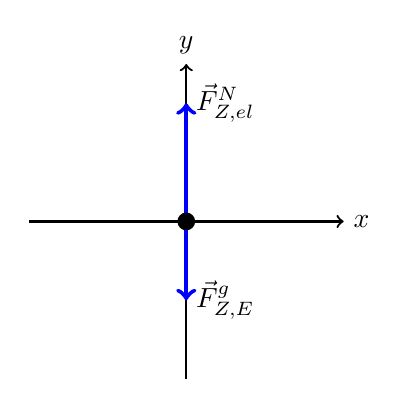
\begin{tikzpicture}
		\FBDaxes{0,0}{0}{axes}
		\FBDvectorXY{axes}{0,1.5}{FN}
		\node[anchor=west] at (FNtip) {$\vec{F}^{N}_{Z,el}$};
		\FBDvectorXY{axes}{0,-1}{FG}
		\node[anchor=west] at (FGtip) {$\vec{F}^{g}_{Z,E}$};
		\FBDdot{axes}
	\end{tikzpicture}
\end{figure}

The floor of the elevator pushes up on Zach with the normal force $\vec{F}^{N}_{Z,el}$. In turn, he pushes back on the floor with an equal and opposite force, $\vec{F}^{N}_{el,Z}$ (this is Newton's 3rd law). If the floor were a scale, this is the force that it would measure---it doesn't magically know the force of gravity on Zach, $\vec{F}^{g}_{Z,E}$ (which some might refer to as Zach's actual weight); it can only go off of what it feels from Zach's feet pushing on it. The normal force is Zach's apparent weight.
}
\ProblemSub{\ApparentWeightB}{
(b) What is Zach's apparent weight before the elevator starts braking?
}
\Solution{\ApparentWeightBSol}{
Before braking, the elevator descends at a constant speed. Therefore
\[
\begin{split}
	F^{net}_{y} & = ma_{y} = 0 \\
	F^{N}_{Z,el} - F^{g}_{Z,E} & = 0 \\
	F^{N}_{Z,el} & = F^{g}_{Z,E} = mg = (80\text{ kg})(9.8\text{ m/s}^{2}) \approx 780\text{ N}.
\end{split}
\]
Zach's apparent weight is 780 N while in an inertial reference frame.
}
\ProblemSub{\ApparentWeightC}{
(c) What is Zach's apparent weight while the elevator is braking?
}
\Solution{\ApparentWeightCSol}{
The elevator must decelerate from 12 m/s to 0 m/s over 3.0 seconds. On average, that means
\[
a_{y} = \frac{\Delta v}{\Delta t} = \frac{12\text{ m/s}}{3.0\text{ s}} = 4.0 \text{ m/s}^{2}.
\]
Now, the net force is nonzero, and we find
\[
\begin{split}
	F^{net}_{y} & = ma_{y} \\
	F^{N}_{Z,el} - F^{g}_{Z,E} & = ma_{y} \\
	F^{N}_{Z,el} & = ma_{y} + F^{g}_{Z,E} = m(a_{y} + g) = (80\text{ kg})(4.0\text{ m/s}^{2} + 9.8\text{ m/s}^{2}) \approx 1100\text{ N}.
\end{split}
\]
Zach's apparent weight is 1100 N while in the braking elevator.
}
	\Problem{Steady Block on a Sliding Ramp}{\SteadyBlock}{
A block of mass $m$ sits upon a frictionless ramp (inclined at angle $\theta$) that is being pushed to the right. What must the acceleration of the ramp be to prevent the block from sliding down the surface?
}
\ProblemFig{\SteadyBlockFig}{
\centering
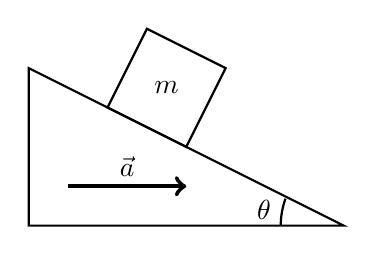
\begin{tikzpicture}
	\draw[thick] (0,0) -- (4,0) -- (0,2) -- cycle;
	\draw[thick] (3.2,0) arc (180:160:1);
	\node[anchor=east] at (3.2,0.2) {$\theta$};
	\draw[thick] (1,1.5) -- (2,1) -- (2.5,2) -- (1.5,2.5) -- cycle;
	\node at (1.75,1.75) {$m$};
	\draw[ultra thick,->] (0.5,0.5) -- (2,0.5);
	\node[anchor=south] at (1.25,0.5) {$\vec{a}$};
	\if\GrayProb1
	\draw (4,1) -- (6,1);
	\node[anchor=west] at (6,1) {$x$};
	\draw (5,0) -- (5,2);
	\node[anchor=south] at (5,2) {$y$};
	\draw[thick] (5,1.5) arc (90:71:0.8);
	\node[anchor=west] at (4.95,1.7) {$\theta$};
	\draw[ultra thick,blue,->] (5,1) -- (5.5,2);
	\node[anchor=west] at (5.5,2) {$\vec{F}^{N}_{BR}$};
	\draw[ultra thick,blue,->] (5,1) -- (5,0);
	\node[anchor=south west] at (5,0) {$\vec{F}^{g}_{BE}$};
	\filldraw[black] (5,1) circle (4pt);
	\draw[ultra thick,red,->] (4.25,1.5) -- (4.75,1.5);
	\node[anchor=south] at (4.5,1.5) {$\vec{F}_{net}$};
	\fi
\end{tikzpicture}
}
\Solution{\SteadyBlockSol}{

If the block is not sliding down the surface of the ramp, then it is moving with it, so the acceleration of the block must be the same as that of the ramp, which points directly to the right. Since we know the direction of acceleration, it will be advantageous to set up our coordinate system with one of the axes along that direction. This differs from several other ramp problems, where a tilted coordinate system is advantageous due to there being fewer vectors to break into components.

If acceleration is along the $x$-axis, as depicted above, we need the two forces (the force on the block normal to the surface of the ramp and the force of gravity on the block) to cancel in the $y$-direction. As such,
\[
0=F^{N}_{BR,y}+F^{g}_{BE,y}=F^{N}_{BR}\cos\theta-mg \implies F^{N}_{BR}\cos\theta=mg \implies F^{N}_{BR}=\frac{mg}{\cos\theta}.
\]
Meanwhile, in the $x$-direction, we only have the $x$-component of the normal force, so
\[
F_{net,x} = F^{N}_{BR,x} = F^{N}_{BR}\sin\theta = mg\frac{\sin\theta}{\cos\theta} = mg\tan\theta.
\]
Since $F_{net,x}=ma_{x}=ma$, we can cancel out the mass to obtain
\[
a = g\tan\theta.
\]
In the special case of a flat ramp, which we expect does not need to move to keep the box from sliding, we have $\theta=0$, and thus $\tan\theta=0$, so our equation indeed gives us $a=0$. Alternatively, if the ramp is vertical, then we cannot keep the block from sliding, as there is nothing beneath it to hold it up. This is the $\theta\to90^{\circ}$ case, and that gives us $a=g\tan\theta\to\infty$, since there is not a finite acceleration sufficient to hold up the block.
}
\end{document}